\def\mitem{\medskip\item}
\def\fitem#1#2{\textcolor{hard}{\small (#1)}~~#2 \medskip \\}
\def\fpitem#1#2{\phantom{\small (#1)}~~#2 \medskip \\}

\begin{frame} \frametitle{Description of data structure}
\begin{definition}
	A cell is \emph{big} if it has size at least $N^{\frac14}$. Otherwise it is \emph{small}.
\end{definition} \bigskip \pause

\begin{center} \begin{tabular}{lcc}
\makecell[l]{
	\fitem{1}{Graph of VD in a form of adjacency list,}
	\fitem{2}{{\it Dynamic nearest neighbor} structure for sites,}
	\fitem{3}{Graph of big cells stored as adjacency list,}
	\fitem{4}{For each big cell:}
	\fpitem{4}{–~linked list of DCRs,}
	\fpitem{4}{–~binary search tree of vertices in circular order.}
} & \hspace{-0.95cm} &
	\makecell[c]{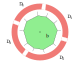
\includegraphics[width=4.5cm]{figs/consecDataStr}}
\end{tabular}
\end{center}
\end{frame}

\def\lrp#1{\left( #1 \right)}
\def\lrc#1{\left\lceil#1\right\rceil}
\def\otl{$\Ot(1)$ } \def\Ot{\tilde O}
\newcommand{\nof}{N^\frac{1}{4}}
\newcommand{\noh}{N^\frac{1}{2}}
\newcommand{\ntf}{N^\frac{3}{4}}

\begin{frame} \frametitle{Handling insertion}
\vspace{-7mm}
\begin{block}{\vspace*{-3ex}}
	Initialize queue; look at cells one-by-one, on each step add to it \\
	unprocessed cells with changes, then implement changes.
\end{block} \pause

\begin{itemize}
	\item Small cell: look at each paw to find neighboring cells needing changes, \\
	    add them to the queue.
	\mitem Big cell: ask DCRs to return Voronoi circles that enclose $s_N$, \\
	    add corresponding cells to the queue.
\end{itemize} \vspace{-2mm} \pause

\begin{block}{\vspace*{-3ex}} \vspace{-3.6mm}
{\small $$\text{Time complexity:\quad}
\Ot \lrp{
s\nof +
\sum_{i=1}^{|B|}  \lrp{ \lrc{\frac{|b_i|}{\nof }}+\ell_i}
+ \ntf + s\nof
}.
$$} \vspace{-2.6mm} \pause

\centerline{This is $\Ot(\ntf)$ amortized.}
\end{block}
\end{frame}